
\chapter{Implementierung}\label{chap:implementierung}

Das Kernziel des Projektes ist es, die formale Notation der operationellen Semantik in eine ausführbare Implementierung umzuwandeln.
Die Wahl der Implementierungssprache fällt hier auf Java, eine imperative und objektorientierte Programmiersprache.
Als Notation zur Beschreibung der Semantik werden in~\cite{Jones_StockHardwareSTG} Zustandsübergänge gewählt, welche in Schreibweise einer Funktion auf bestimmte Muster des Maschinenzustands greifen und auf den nächsten Zustand der Ausführung abbilden.
Diese Notation kann nicht ohne Weiteres in die imperative Programmiersprache Java übersetzt werden.
Doch genau hier liegt der Reiz des Projektes, da die \gls{stg} genau für diesen Zweck gedacht ist, die semantische Lücke zwischen verzögert ausgewerteten funktionalen Hochsprachen und dem hardwarenahen imperativen Ausführungsmodell herkömmlicher Hardware zu schließen.
Zwar wird Java kaum als hardwarenahe Programmiersprache verwendet, die imperativen Eigenschaften sind jedoch vorhanden und Features wie Objektorientierung und automatische Speicherverwaltung unterstützen die zielgerichtete Implementierung.

\section{Der Maschinenzustand}

Der Zustand der \gls{stg}-Maschine besteht aus insgesamt fünf Komponenten, die in Java abgebildet werden:

\begin{enumerate}
\item Der \textit{Maschinencode}, welcher eine feste Anzahl an Ausprägungen annehmen kann,
\item der \textit{Argument-Stack}, welcher Werte enthält,
\item der \textit{Return-Stack}, welcher \textit{Continuations} speichert,
\item der \textit{Update-Stack}, welcher Informationen zur Ersetzung von Closures speichert, und
\item der \textit{Heap}, welcher die Closures speichert.
\end{enumerate}

Zudem existiert eine statische, globale Umgebung, welche die Adressen für alle Closures liefert, die auf oberster Programmebene definiert sind.
Diese Umgebung ist während der gesamten Laufzeit unverändert.

Die drei verschiedenen Stacks werden als \texttt{Deque} aus dem Paket \texttt{java.util} dargestellt.
Für die Elemente, die diese Stacks speichern, werden verschiedene Klassen angelegt, um die einzelnen Ausprägungen darzustellen.
Continuations und die Informationen zur Ersetzung von Closures (genannt Update-Rahmen) werden jeweils als Records in Java dargestellt.

Für Werte, die auf dem Argument-Stack liegen, existieren zwei Ausprägungen: Ganzzahlen und Adressen.
Es wird für beide jeweils ein Java-Record erstellt, welcher einer gemeinsame Schnittstelle implementiert.

\begin{lstlisting}[language=java, morekeywords={record, sealed}, caption={Darstellung von Werten in Java}, label={lst:value}]
public sealed interface Value {
  record Address(int address) implements Value {}

  record Int(int value) implements Value {}
}
\end{lstlisting}

Ähnlich wird bei den Ausprägungen des Maschinencodes vorgegangen.
Da diese den Zustand der Maschine maßgeblich bestimmen, wird eine Schnittstelle \texttt{State} definiert, die von den verschiedenen Ausprägungen implementiert wird.
Diese Schnittstelle definiert dabei eine Methode \texttt{State transfer(Machine)}, die den nächsten Maschinenzustand zurückgibt.
Auf diese Weise wird das \textit{Tagless}-Verhalten der \gls{stg} simuliert, indem keine expliziten Fallunterscheidungen für den aktuellen Ausführungszustand getroffen werden müssen.
Stattdessen wird polymorph zur richtigen Aktion für den aktuellen Ausführungszustand gesprungen.
Die vier Ausprägungen, die der Maschinencode annehmen kann, sind: \textit{Eval}, \textit{Enter}, \textit{Return Constructor} und \textit{Return Integer}.


\begin{lstlisting}[language=java, morekeywords={record, sealed}, caption={Schnittstelle für die Ausprägungen des Maschinencodes}, label={lst:code}]
public sealed interface State {
    State transfer(final Machine machine);
}
\end{lstlisting}


\section{Auswertung von Atomen}

Um Atome auszuwerten, wird eine Funktion \texttt{val} definiert, die auf die lokale Umgebung $\rho$ und die globale Umgebung $\sigma$ zugreift~\cite{Jones_StockHardwareSTG}.
Diese Funktion wertet eine Konstante zu ihrem Zahlenwert aus und sucht den Wert einer Variablen in der umliegenden Umgebung.
Dabei wird die lokale Umgebung der globalen Vorgezogen.
Die Implementierung dieser Funktion in Java wird \texttt{value} genannt.

\begin{figure}[h]
  \centering
  \[
  val(\rho, \sigma, x) =
    \begin{cases}
      Int\ x & \text{falls}\ x\ \text{eine Konstante} \\
      \rho\ x & \text{falls}\ x\ \in\ dom(\rho) \\
      \sigma\ x & \text{andernfalls}
    \end{cases}
  \]
  \caption{Funktion zur Auswertung von Atomen}\label{fig:val}
\end{figure}



\section{Startzustand}

Der Startzustand beginnt mit der Auswertung der \texttt{main} Funktion, die implizit durch die Maschine aufgerufen wird.

\begin{lstlisting}[language=Java]
private State state = new Eval(
 new FunctionApplication(new Variable("main"), emptyList()),
 emptyMap());
\end{lstlisting}

Die etwas verbose Darstellung in Java beschreibt detailliert den Startzustand:
Es wird mit der Auswertung einer Funktionsanwendung begonnen.
Die angewandte Funktion ist dabei durch die Variable \texttt{main} definiert und besitzt eine leere Parameterliste.
Zudem ist die Umgebung, in der die Auswertung stattfindet, leer.

Die verschiedenen benötigten Stacks werden ebenfalls leer initialisiert.

\begin{lstlisting}[language=java]
private Deque<Value> argumentStack = emptyStack();
private Deque<Continuation> returnStack = emptyStack();
private Deque<UpdateFrame> updateStack = emptyStack();

private final Heap heap = new Heap();
private final Map<Variable, Value> globalEnvironment = allocateAll(heap, program.bindings, emptyMap(), true);
\end{lstlisting}

Letztlich werden Heap und die globale Umgebung auch mit den Standardwerten initialisiert.
Die Implementierung der Funktion \texttt{allocateAll}, welche verwendet wird, um alle globalen Namensbindungen in die globale Umgebung einzutragen und gleichzeitig auf dem Heap anzulegen, wird in Abschnitt~\ref{sec:bindings} näher gezeigt.


\begin{figure}
  \centering
  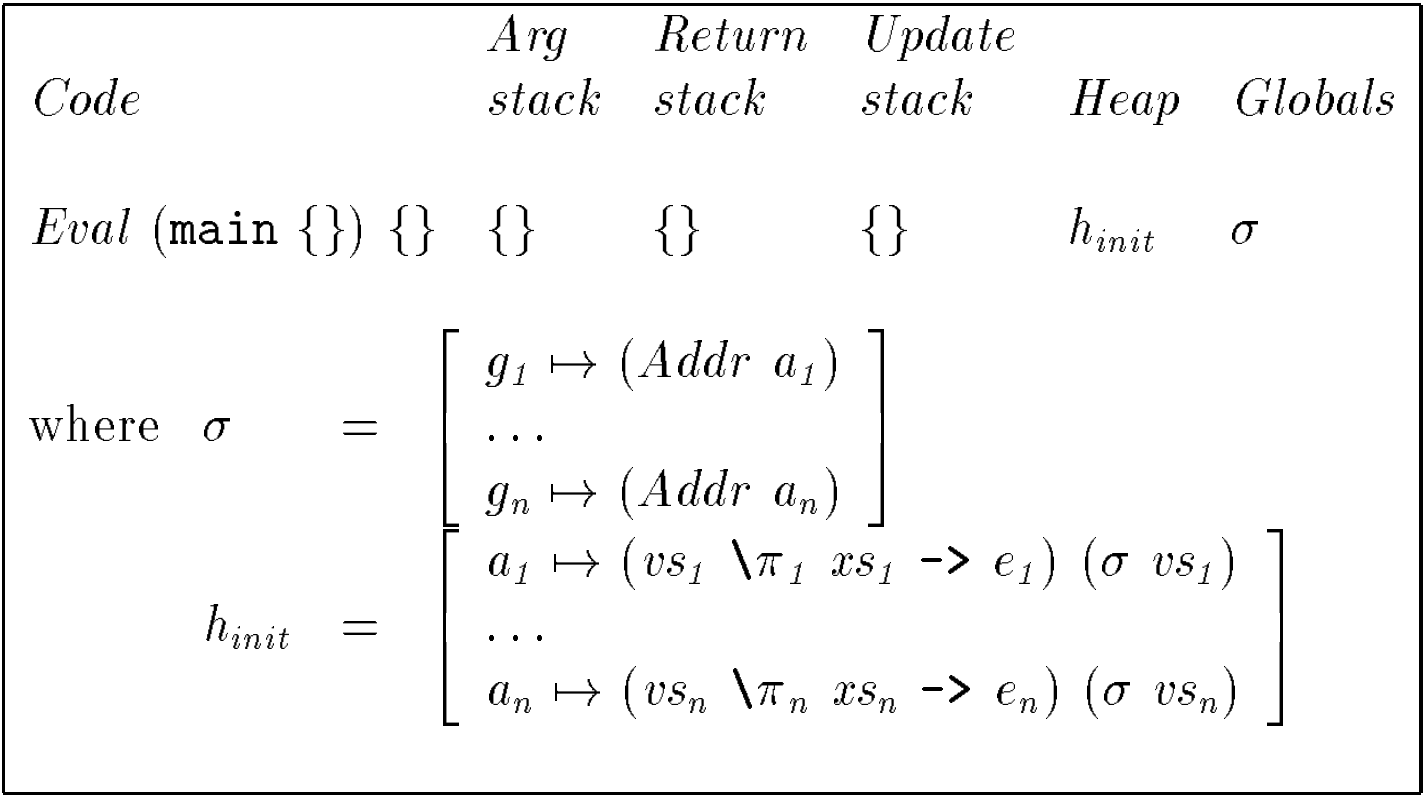
\includegraphics[width=0.9\textwidth]{start-state}
  \caption{Startzustand der Maschine}\label{fig:start-state}
\end{figure}

\section{Funktionsanwendungen}\label{sec:function-applications}

Die Semantik zur Auswertung von Funktionanwendungen wird in~\cite{Jones_StockHardwareSTG} durch Regel~1 und Regel~2 gegeben.
Vor dem Pfeil in dieser Notation steht ein Muster, das die Komponenten des Maschinenzustands gegeben durch Reihenfolge listet: \textit{Maschinencode, Argument-Stack, Return-Stack, Update-Stack}, \textit{Heap} und die globale Umgebung $\sigma$.
Nach dem Pfeil steht der folgende Maschinenzustand.

In der Implementierung in Java wird der Zustand \textit{Eval} durch das Visitor-Muster abgebildet~\cite{Gamma_DesignPatterns}.
Es wird also für jeden möglichen Ausdruck, der ausgewertet werden kann eine \texttt{State visit(\textit{Ausdruck})} Methode implementiert, die eine konkrete Instanz von \texttt{\textit{Ausdruck}} auswertet und den Zustand für den nächsten Auswertungsschritt zurückliefert.

Listing~\ref{lst:visit-function} zeigt die Auswertung von Funktionsanwendungen.
Zunächst wird die Funktion mittels \texttt{value} ausgewertet wird und prüft, ob eine Adresse als Ergebniswert vorliegt.
Ist dies der Fall, werden die Argumente ausgewertet, mit dem Argumentstack konkateniert und ein neuer Zustand zurückgegeben, der die Closure betreten und den darin enthaltenen Code ausführen soll.

\begin{lstlisting}[language=java,caption={Auswertung von Funktionsanwendungen},label={lst:visit-function}]
public State visit(FunctionApplication app) {
  final Value function = value(rho, sigma, app.function);
  if (function instanceof Address a) {
    List<Value> args = values(rho, sigma, app.arguments);
    concat(args, argumentStack);
    return new Enter(a.address());
  }
}
\end{lstlisting}

\begin{figure}[h]
  \centering
  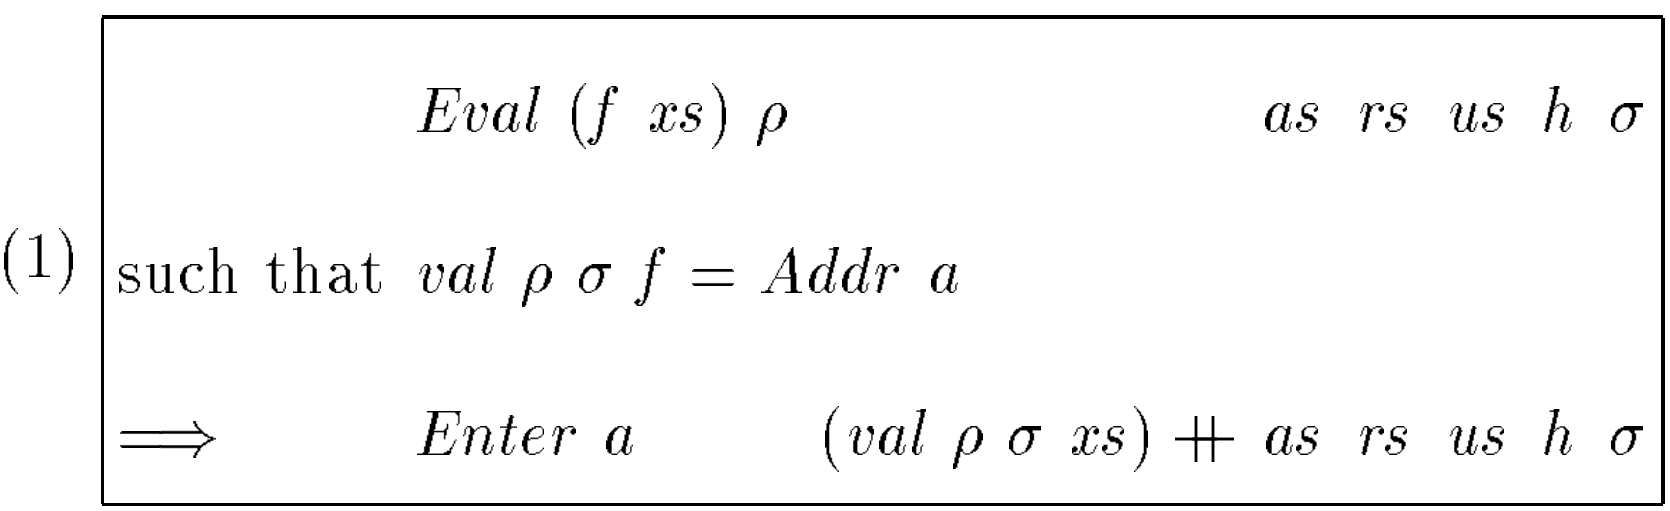
\includegraphics[width=\textwidth]{rule-1}
  \caption{Auswertung von Funktionsanwendungen}\label{fig:rule-1}
\end{figure}


Die zweite relevante Regel für die Auswertung von Funktionsanwendungen beschreibt das Betreten in eine Closure.
Hierbei wird die Closure als Adresse dargestellt und der entsprechende Wert vom Heap geholt.
Wie Abbildung~\ref{fig:rule-2} zeigt, wird für die Auswertung eine lokale Umgebung zusammengestellt.
Diese bildet die Namen der freien Variablen auf die in der Closure gespeicherten Werte und die definierten Parameter auf die Argumente auf dem Argument-Stack ab.
Dabei werden die Werte vom Argument-Stack konsumiert und der Maschinenzustand geht anschließend zur Auswertung des Closure-Rumpfes über.

\pagebreak

\begin{lstlisting}[language=java,morekeywords={record}, caption={Implementierung des Betretens einer Closure}]
public record Enter(int address) implements State {
  public State transfer(final Machine machine) {
    final Closure closure = machine.heap.get(address);

    if (machine.argumentStack.size()
         >= closure.code().parameters.size()) {
      final var rho = mkLocalEnv(...);
      return new Eval(closure.body(), rho);
    }
  }
}
\end{lstlisting}

\begin{figure}[h]
  \centering
  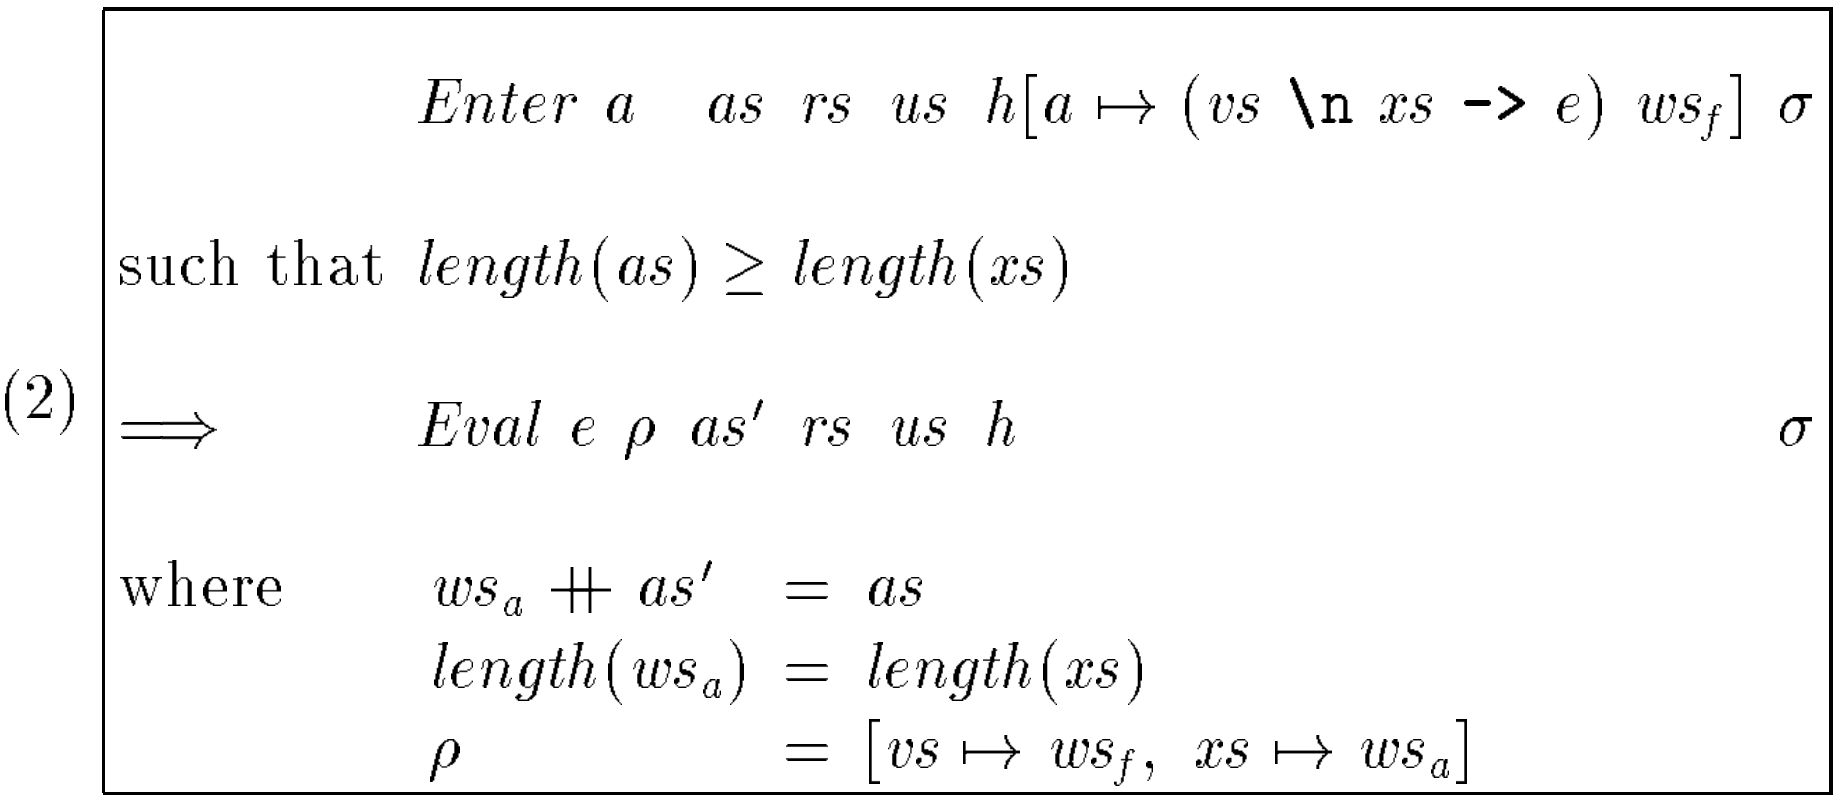
\includegraphics[width=\textwidth]{rule-2}
  \caption{Betreten einer Closure}\label{fig:rule-2}
\end{figure}

\section{Namensbindungen}\label{sec:bindings}

In der \gls{stg}-Sprache sind Namensbindungen für Speicherallokation zuständig.
Folglich ist dies ein großer Aufgabenteil bei der Auswertung von Namensbindungen.
Zusätzlich muss den innere Ausdruck der Namensbindung ausgewertet werden und die Umgebung für diesen aufgebaut.

In Abbildung~\ref{fig:stg-rule3} wird Regel~3 aus~\cite{Jones_StockHardwareSTG} dargestellt.
Im dargestellten Fall, der die Auswertung von nicht-rekursiven Namensbindungen mit \texttt{let} beschreibt, ist es möglich, die drei Aufgabenteile strikt zu trennen.
Für rekursive Namensbindungen mit \texttt{letrec} ist dies nicht möglich, da dann $\rho_{rhs}\ =\ \rho'$ gilt und das Aufbauen der Umgebung mit dem Anlegen der Closures auf dem Heap verzahnt ist.
Um die durch den Ausdruck definierten Closures zu erstellen, müssen die Adressen aller im Ausdruck definierter Closures bekannt sein.
Damit eine Closure auf den Heap gelegt werden kann, muss diese jedoch erstellt sein.

\begin{figure}[h]
  \centering
  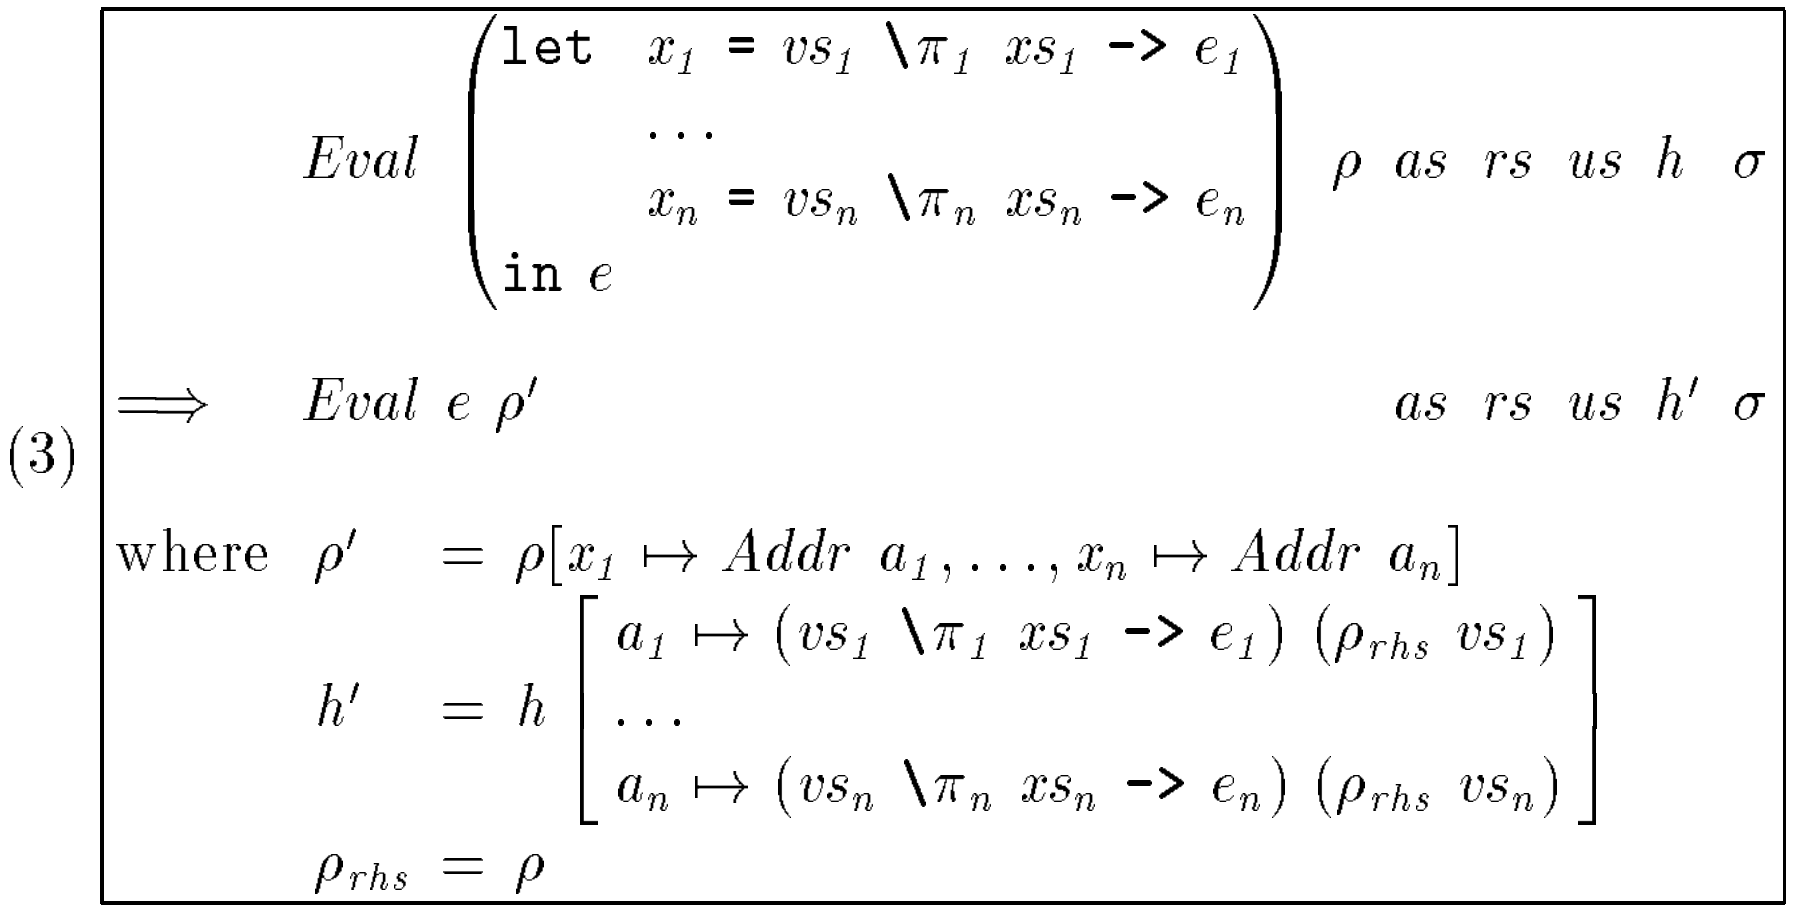
\includegraphics[width=0.95\textwidth]{rule-3}
  \caption{Regel zur Auswertung von Namensbindungen}\label{fig:stg-rule3}
\end{figure}


Als Lösung für diese gegenseitige Abhängigkeit wird die Funktion \texttt{allocateAll} aus Listing~\ref{lst:allocate-all} verwendet.
Die Auswertung von Namensbindungen ist mit Hilfe der Funktion \texttt{allocateAll} trivial:

\begin{lstlisting}[language=java]
public State visit(LetBinding let) {
  final var env = allocateAll(heap, let.bindings, rho, let.isRecursive);
  return new Eval(let.expression, env);
}
\end{lstlisting}

Die Funktion \texttt{allocateAll} akzeptiert den Heap, eine Liste aus Namensbindungen und eine Umgebung, in der die Namensbindungen stattfinden als Parameter.
Zusätzlich wird angegeben, ob die Namensbindung rekursiv erfolgen soll.
Als Effekt legt diese Funktion Closures für die zu bindenen Namen auf dem Heap an und gibt anschließend eine Umgebung zurück, in der die gebundenen Namen sichtbar sind.
Die gewählte Strategie hierfür ist, für jeden Namen eine Adresse auf dem Heap zu reservieren.
Die jeweilige Adresse genügt, damit die gebundenen Namen aufeinander verweisen können.
Anschließend wird die Eigenschaft der \gls{stg} ausgenutzt, Closures auf dem Heap aktualisieren zu können (siehe Abschnitt~\ref{sec:updateable-closures}).
Die nun erstellten Closures werden an die jeweils reservierte Adresse im Heap platziert.
In der Implementierung taucht ein Kombinator \texttt{combineWith} auf, welcher zwei iterierbare Strukturen akzeptiert sowie eine Funktion, die paarweise auf die Elemente der beiden Datenstrukturen angewandt wird.
Durch ihn werden die reservierten Adressen mit den Namen und erstellten Closures verbunden.

\vfill

\begin{lstlisting}[language=java, caption={Funktion \texttt{allocateAll} zum Anlegen rekursiver Namensbindungen}, label={lst:allocate-all}]
private static Map<Variable, Value> allocateAll(
  final Heap heap, final List<Bind> bindings,
  final Map<Variable, Value> outerEnvironment,
  final boolean isRecursive) {
  // Lokale Umgebung wird erstellt mit allen sichtbaren Namen der umliegenden Umgebung.
  final var localEnvironment =
    new HashMap<>(outerEnvironment);

  // Reserviere die Adressen aller Definitionen und trage sie in der Umgebung ein.
  final Iterable<Integer> addresses = heap.reserveMany(bindings.size());
  combineWith(addresses, bindings, (addr, bind) -> {
    localEnvironment.put(bind.variable, new Address(addr))
  });

  final var rhsEnvironment = (isRecursive) ? localEnvironment : outerEnvironment;

  // Aktualisiere Closures im Heap.
  combineWith(addresses, bindings, (address, bind) -> {
    List<Value> capturedValues = new ArrayList<>();
    for (Variable free : bind.lambda.freeVariables())
      capturedValues.add(rhsEnvironment.get(free));

    heap.update(address,
      new Closure(bind.lambda, capturedValues));
  });
  return localEnvironment;
}
\end{lstlisting}

\vfill


\section{Fallunterscheidungen}

Wird im Auswertungszustand der Maschine auf eine Fallunterscheidung als Ausdruck getroffen, wird nicht sofort zur passenden Alternative gesprungen.
Die Alternativen werden lediglich als Continuation auf den \textit{Return-Stack} geschoben und Maschine führt mit der Auswertung des untersuchten Ausdrucks fort.

\begin{figure}[h]
  \centering
  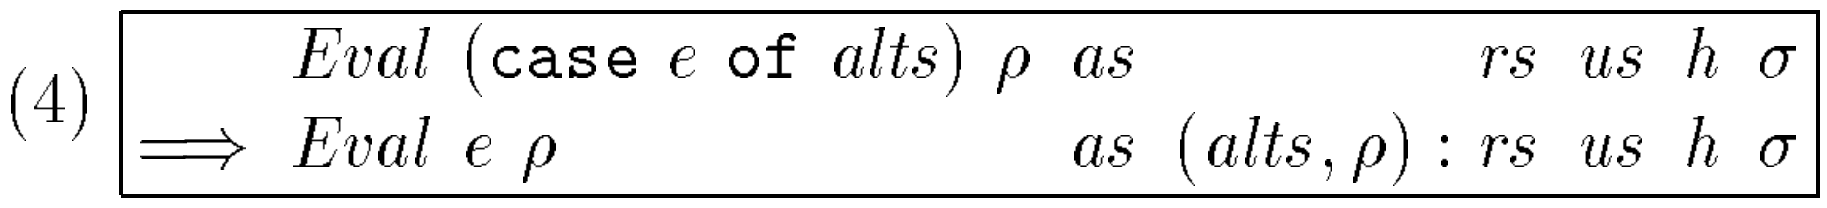
\includegraphics[width=0.8\textwidth]{rule-4}
  \caption{Regel zur Auswertung von Fallunterscheidungen}\label{fig:rule-4}
\end{figure}

Die Implementierung in Java schiebt ebenso nur eine Continuation auf den Stack und gibt den neuen Maschinenzustand als Ergebnis zurück.

\begin{lstlisting}[language=java]
public State visit(CaseExpression expression) {
  returnStack.push(
      new Continuation(expression.alternatives, rho));
  return new Eval(expression.scrutinized, rho);
}
\end{lstlisting}

Die tatsächliche Auswahl einer Alternative geschieht erst nachdem die Auswertung des untersuchten Ausdrucks abgeschlossen ist.
Dann einen speziellen Zustand übergegangen, um zur Fallunterscheidung zurückzukehren.
Dieser Zustand tritt ein, wenn die Anwendung eines Konstruktors ausgewertet wird, wie die Regel in Abbildung~\ref{fig:rule-5} zeigt.

\begin{figure}[h]
  \centering
  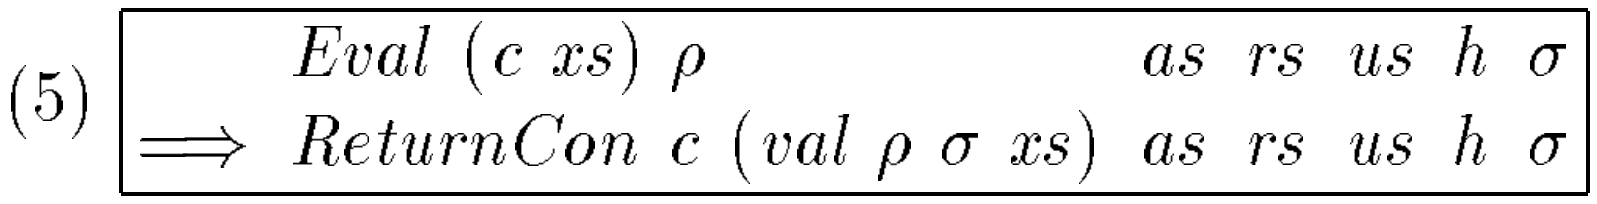
\includegraphics[width=0.8\textwidth]{rule-5}
  \caption{Regel zur Auswertung von Konstruktoranwendungen}\label{fig:rule-5}
\end{figure}

Abbildungen~\ref{fig:rule-6},~\ref{fig:rule-7}~und~\ref{fig:rule-8} zeigen die involvierten Regeln zur Auswahl einer Alternative.
Da diese drei Regeln zusammen wirken, um die korrekte Alternative auszuwählen, werden sie zu einer Methode in Java zusammengefasst.
Die Continuation wird zunächst vom Stack entfernt und anschließend die darin gespeicherten Alternativen der Reihe nach untersucht, ob deren Konstruktor dem Konstruktor aus dem Maschinenzustand entspricht.
Falls eine passende Alternative gefunden wird, werden die Variablen der Alternative entsprechend Regel~6 gebunden und die in die Auswertung des Ausdrucks der Alternative übergegangen.
Auf diese Weise wird die Schleife über die Alternativen vorzeitig abgebrochen.

Besitzt jedoch keine der Alternativen einen passenden Konstruktor, so wird die Standardalternative untersucht.
Zunächst wird auf den Fall aus Regel~8 geprüft.
Tritt dieser auf, wird das gesamte Ergebnis der Auswertung an einen Namen gebunden statt lediglich einzelne Variablen zu extrahieren.
Dafür muss eine Closure angelegt werden, die den Konstruktor und die angewandten Werte speichert.
Regel~7 hingegen bindet keinen Namen und setzt die Ausführung wie in Regel~8 mit der Auswertung des Ausdrucks aus der Alternative fort.

\vfill

\begin{lstlisting}[language=java, morekeywords={record, var}, caption={Implementierung der Auswahl einer Alternative}]
public record ReturnConstructor(Constructor constructor,
                List<Value> arguments) implements State {
  public State transfer(Machine machine) {
    final var continuation = machine.returnStack.pop();

    // Suche nach passender Alternative.
    for (Alternative alt : continuation.alternatives())
      if (areEqual(this.constructor, alt.constructor)) {
        // Passende Alternative gefunden.
        combineWith(alt.arguments, this.arguments,
          continuation.savedEnvironment()::put);
        return new Eval(alt.expression,
          continuation.savedEnvironment());
      }

    // Verwende Standard-Alternative.
    if (continuation.defaultAlternative()
         instanceof DefaultBindingAlternative def) {
      Address address = machine.heap
        .allocate(standardConstructorClosure());
      continuation.savedEnvironment()
        .put(def.variable, address);
      return new Eval(def.expression,
        continuation.savedEnvironment());

    } else if (continuation.defaultAlternative()
         instanceof DefaultFallthroughAlternative def) {
      return new Eval(def.expression,
        continuation.savedEnvironment());
    }
  }
}
\end{lstlisting}

\vfill

\pagebreak

\begin{figure}[h]
  \centering
  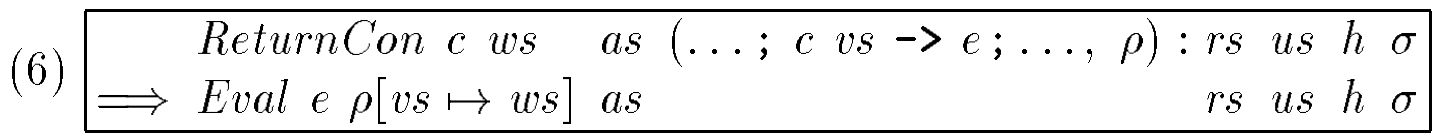
\includegraphics[width=0.9\textwidth]{rule-6}
  \caption{Regel zur Auswahl einer Alternative}\label{fig:rule-6}
\end{figure}

\begin{figure}[h]
  \centering
  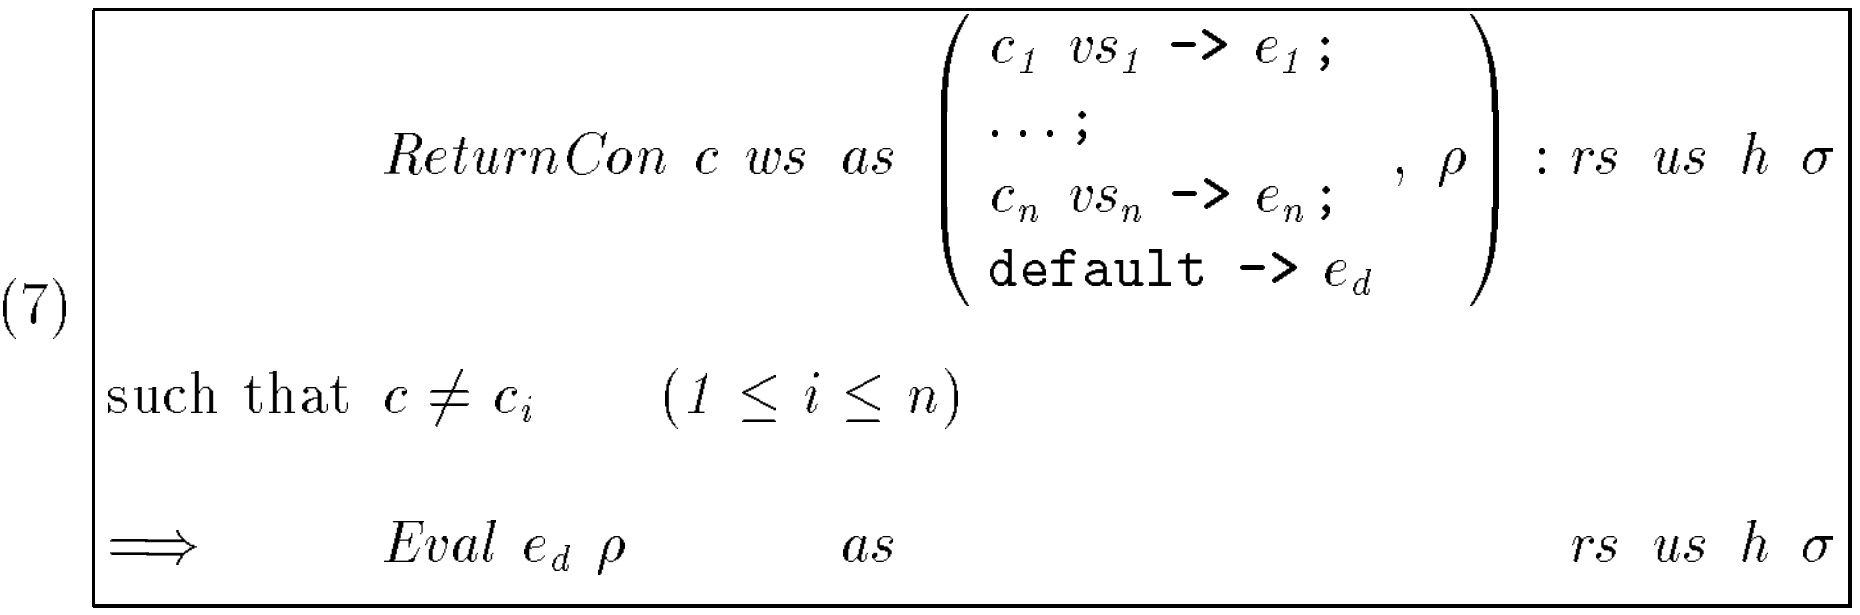
\includegraphics[width=0.9\textwidth]{rule-7}
  \caption{Regel zur Auswahl der Standardalternative}\label{fig:rule-7}
\end{figure}

\begin{figure}[h!]
  \centering
  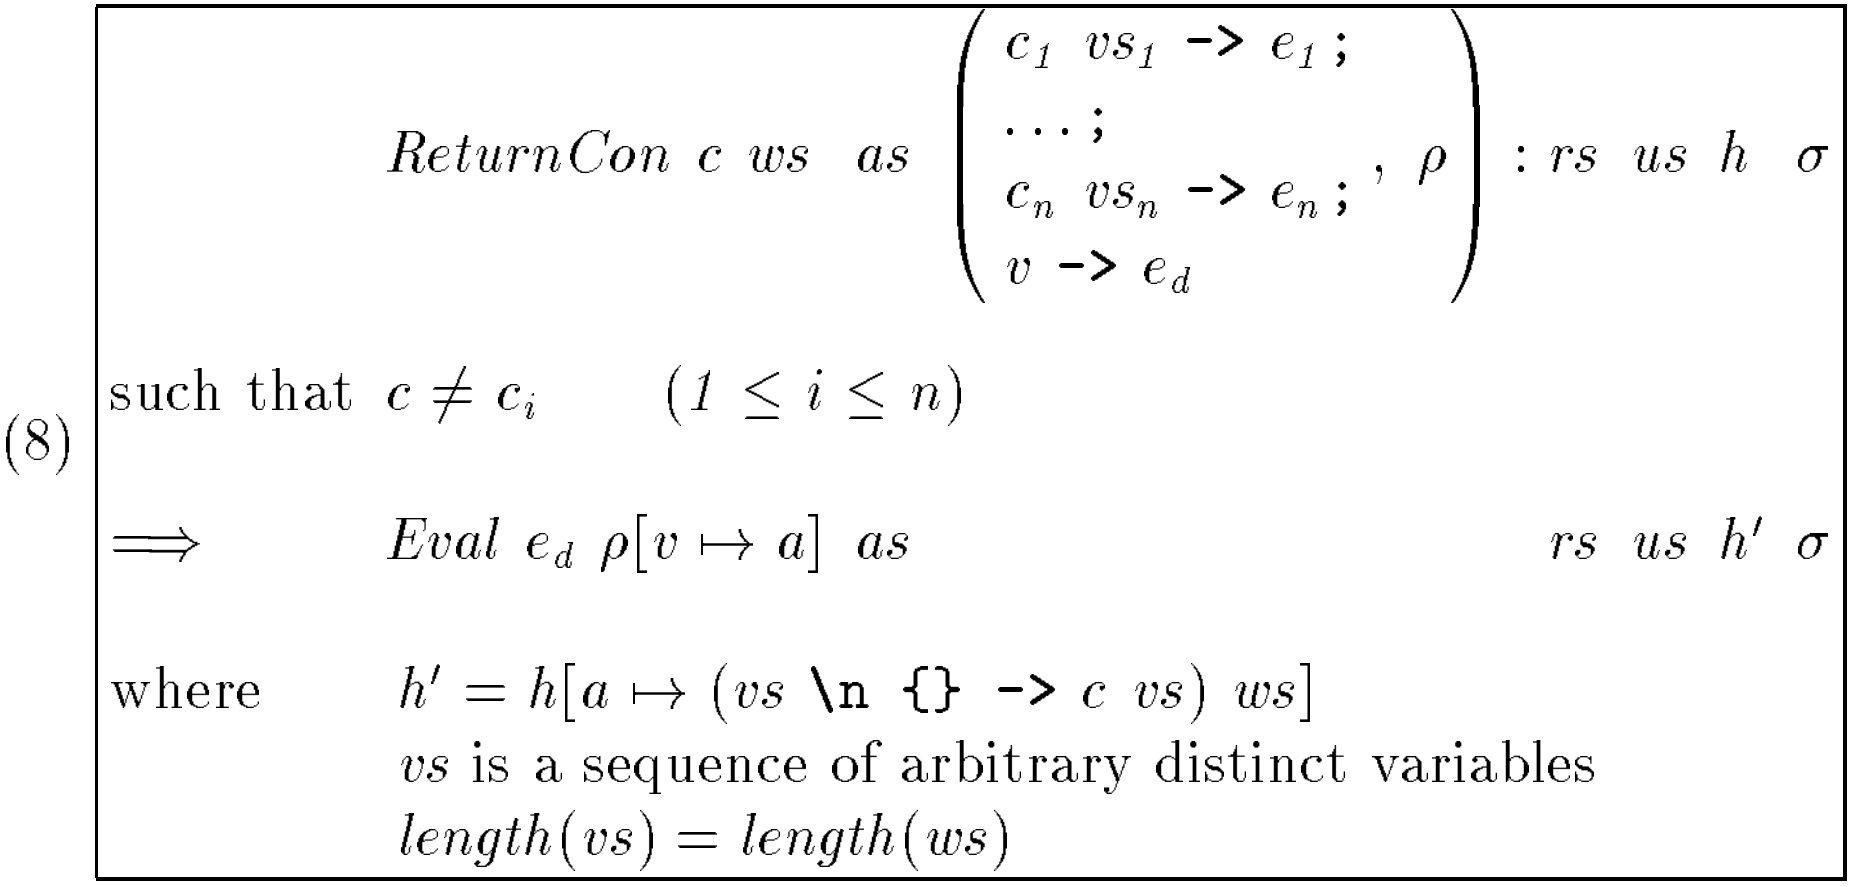
\includegraphics[width=0.9\textwidth]{rule-8}
  \caption{Regel zur Auswahl der Standardalternative mit Namensbindung}\label{fig:rule-8}
\end{figure}

Für primitive Zahlenwerte wird ein ähnlicher Zustand \texttt{ReturnInt} bereitgestellt, welcher sich analog zu \texttt{ReturnConstructor} verhält.
Statt die verschiedenen Alternativen auf passende Konstruktoren zu überprüfen, wird nach einem passenden Zahlenwert gesucht (Regel~11).
Die Regeln zur Auswahl von Standardalternativen (Regel~12 und Regel~13) sind äquivalent zu denen im Zustand \texttt{ReturnConstructor}.
Die einzige Besonderheit bei der Auswertung von primitiven Zahlenwerten ist, dass die Auswertung einer Variable, die einen primitiven Zahlenwert speichert, in den Zustand \texttt{ReturnInt} übergeht.
Dies erklärt die Einschränkung in Abbildung~\ref{fig:rule-1} aus Abschnitt~\ref{sec:function-applications}.


\section{Aktualisierbare Closures}\label{sec:updateable-closures}

Zum Aktualisieren von Closures auf dem Heap müssen mehrere Regeln zusammenspielen.
Einerseits wird beim Betreten einer aktualisierbaren Closure ein entsprechender Rahmen auf den Update-Stack geschoben.
Andererseits muss der Rahmen vom Stack wieder entfernt werden, wenn ein Update ausgelöst wird.

\begin{figure}[h]
  \centering
  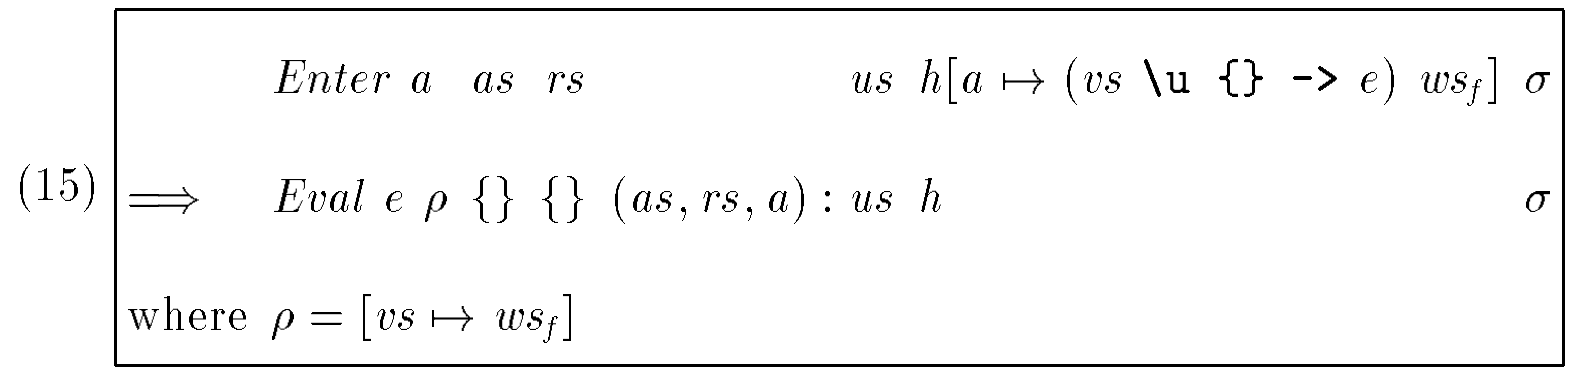
\includegraphics[width=0.95\textwidth]{rule-15}
  \caption{Regel zum Betreten einer aktualisierbaren Closure}\label{fig:rule-15}
\end{figure}

Regel~15 in Abbildung~\ref{fig:rule-15} stellt das Betreten einer aktualisierbaren Closure dar.
Diese Regel ist ähnlich zur Regel zum Betreten einer nicht-aktualisierbaren Closure mit dem Unterschied, dass ein Update-Rahmen auf den entsprechenden Stack gelegt wird.
Das Erstellen dieses Rahmens leert den Argument- und Return-Stack.
Die Inhalte beider Stacks werden im Rahmen gespeichert zusammen mit der Adresse der aktualisierbaren Closure.
Dieses Verhalten lässt sich durch Anpassen der existierenden Implementierung mit minimalen Aufwand erreichen, indem eine einzelne Verzweigung ergänzt wird:

\begin{lstlisting}[language=java]
if (closure.code().isUpdateable) {
  machine.updateStack.push(new UpdateFrame(
    machine.argumentStack, machine.returnStack, address));
  machine.argumentStack = emptyStack();
  machine.returnStack = emptyStack();
}
 ...
\end{lstlisting}

Der schwierigere Teil ist das Anwenden einer Aktualisierung, wenn die Auswertung einer aktualisierbaren Closure abgeschlossen ist.
Es existieren zwei Fälle, in denen der Abschluss einer Auswertung erkannt und somit deine Aktualisierung ausgelöst wird.

\begin{enumerate}
\item
  Wird der Wert einer Closure als Konstruktor bekannt, so folgt anschließend der Versuch, eine Continuation vom Return-Stack zu holen, um die Auswahl einer Alternative auszuführen.
  Wenn der Return-Stack leer ist, kann dieser Versuch nur scheitern.
  Diese Situation wird dann als Aktualisierung erkannt.
\item
  Ist der Wert einer Closure eine Funktion, versucht diese die Funktionsargumente vom Argument-Stack zu konsumieren.
  Sind keine Argumente auf dem Stack vorhanden, so scheitert dieser Versuch ebenso, was als Aktualisierung erkannt wird.
\end{enumerate}

Diese beiden Ereignisse werden als Regel~16 und Regel~17 dargestellt.

\begin{figure}[h]
  \centering
  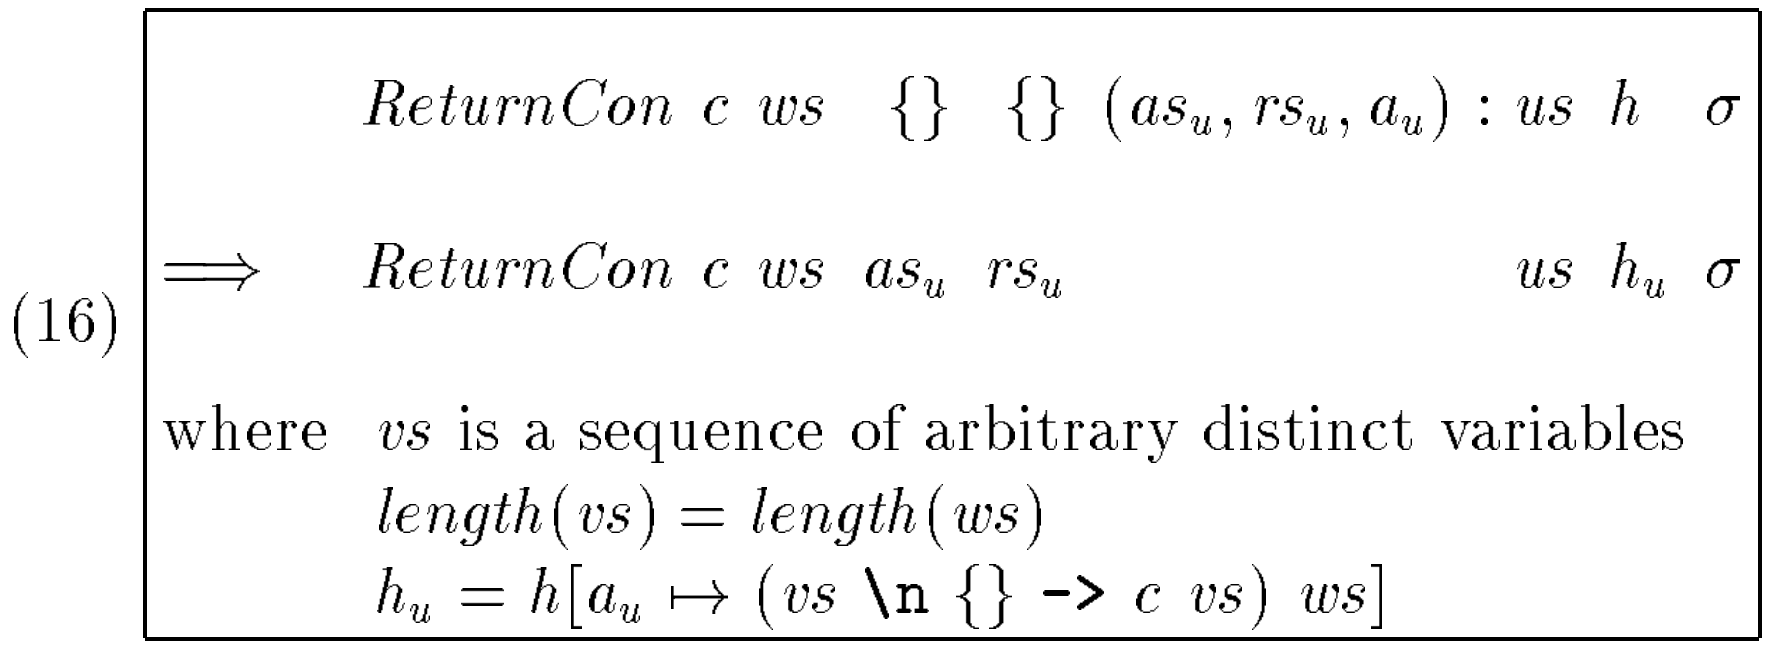
\includegraphics[width=0.9\textwidth]{rule-16}
  \caption{Regel zur Erkennung von Aktualisierungen bei Konstruktoren}\label{fig:rule-16}
\end{figure}

\begin{figure}[h]
  \centering
  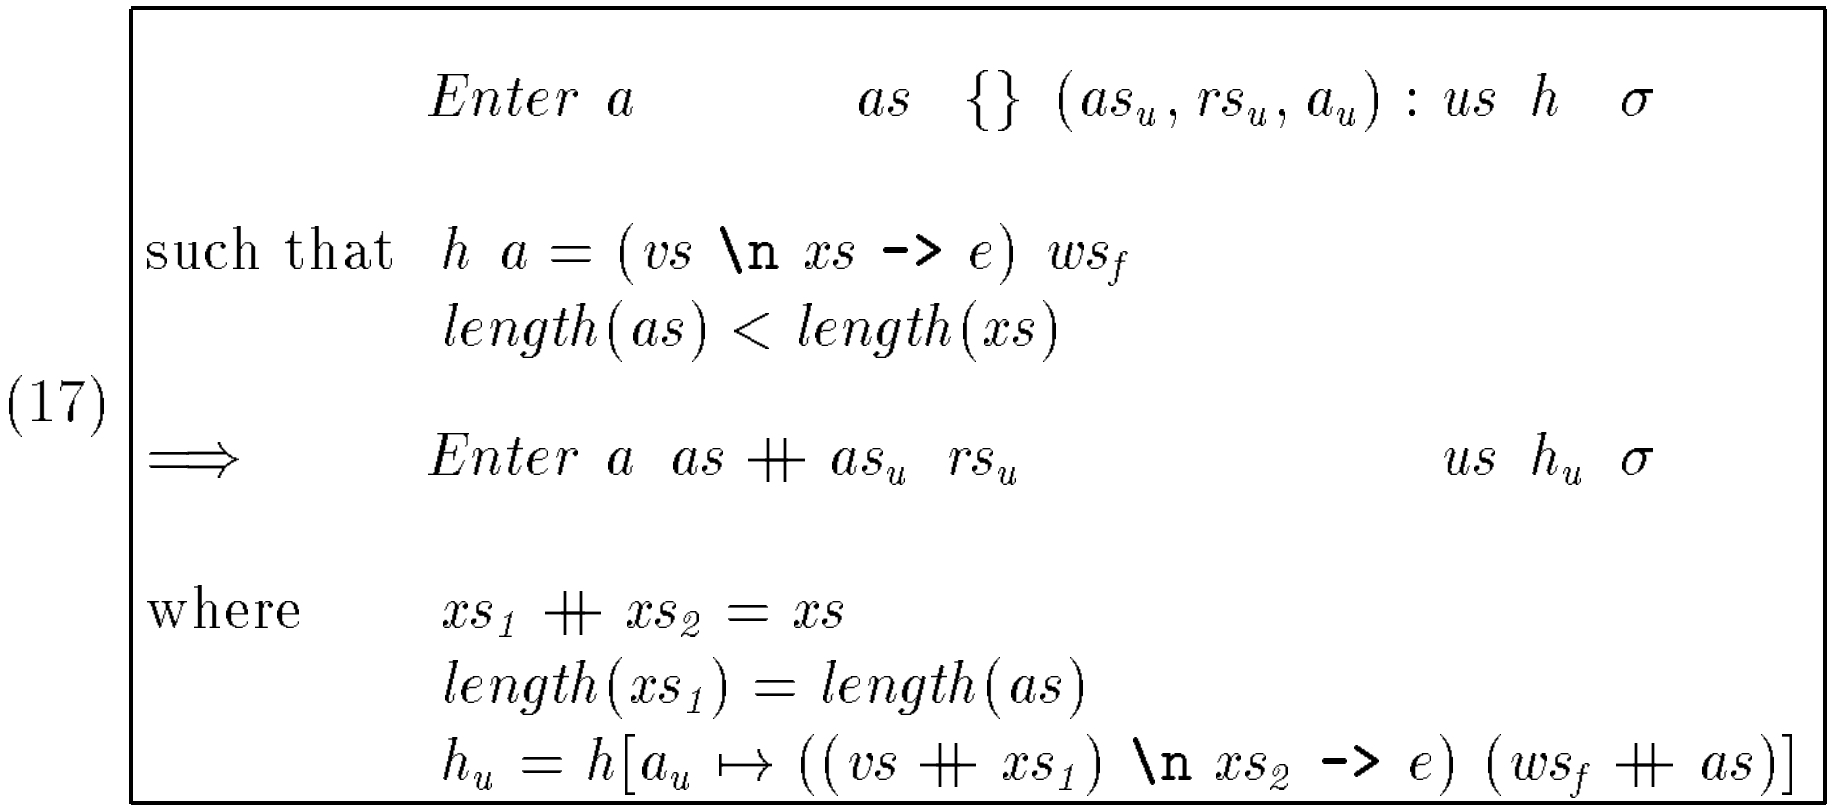
\includegraphics[width=0.9\textwidth]{rule-17}
  \caption{Regel zur Erkennung von Aktualisierungen bei Funktionen}\label{fig:rule-17}
\end{figure}

Wie bereits zu erkennen ist, sind diese Regeln vergleichsweise komplex und benötigen einige Hilfsdefinitionen, die größtenteils dazu dienen, die Stacks korrekt wiederherzustellen und die korrekte Anzahl an Werten für den Folgezustand zur Verfügung zu stellen.
Um beide Fälle in der Implementierung zu erkennen, wird jeweils eine Verzweigung ergänzt.

Listing~\ref{lst:rule-16} stellt dar, wie im Zustand \texttt{ReturnConstructor} überprüft wird, ob der Return-Stack ein Element zum Entfernen enthält (siehe Regel~16).
Ist dies nicht der Fall, wird der Konstruktor samt Parameter bei der Ersetzung eingesetzt.
Der Code zum Einrichten der Closure ist hierbei identisch zu dem, der ausgeführt wird, wenn die Standardalternative im Zustand \texttt{ReturnConstructor} einen Namen bindet.

\begin{lstlisting}[language=java, caption={Erkennung von Aktualisierungen bei Konstruktoren}, label={lst:rule-16}]
if (machine.returnStack.isEmpty()) {
  final UpdateFrame frame = machine.updateStack.pop();

  machine.argumentStack = frame.argumentStack();
  machine.returnStack = frame.returnStack();
  machine.heap.update(frame.address(), standardConstructorClosure());

  return this;
}
\end{lstlisting}

Bei der Übersetzung von Regel~17, wie sie in Listing~\ref{lst:rule-17} zu sehen ist, wird ein großteil der Codezeilen für die Manipulation der verschiedenen Listen verwendet.
Was sich als Muster kurz und präzise ausdrücken lässt, lässt sich in Java lediglich über das Zusammenspiel von mehreren Listenprimitiven implementieren.
Da diese Codezeilen nur schwer nachvollziehbar sind und Abbildung~\ref{fig:rule-17} bereits deren Bedeutung darstellt, werden sie hier weggelassen.
Die Closure, die zur Ersetzung erstellt wird, kopiert dabei den Rumpf aus der Continuation.
Lediglich Parameter, freie Variablen und deren Werte werden angepasst.

\begin{lstlisting}[language=java, caption={Implementierung der Erkennung von Aktualisierungen bei Funktionen}, label={lst:rule-17}]
if (machine.argumentStack.size() < closure.code().parameters.size()) {
  final List<Variable> parameters = ...;
  final List<Variable> freeVariables = ...;
  final List<Value> boundValues = ...;

  final UpdateFrame frame = machine.updateStack.pop();
  machine.returnStack = frame.returnStack();
  machine.argumentStack.addAll(frame.argumentStack());

  machine.heap.update(frame.address(), new Closure(...));
  return this;
}
\end{lstlisting}


Als Besonderheit bei diesen beiden Regeln ist festzustellen, dass sich die Code-Komponente nicht ändert.
Bei der Implementierung in Java wird dies besonders deutlich, da \texttt{return this} den nächsten Codezustand und somit den aktuellen Zustand unverändert bereitstellt.
Grund dafür ist, dass der Wert, der durch die Aktualisierung einer Closure entsteht, das Ergebnis einer anderen aktualisierbaren Closure sein könnte.
Daher wird erneut auf die verschiedenen Fälle geprüft, um eventuell eine weitere Closure zu aktualisieren.


\section{Ausführung}\label{sec:runtime}

Da die Code-Komponente der Maschine \textit{tagless} mit Hilfe des Polymorphismus in Java implementiert wurde, ist die tatsächliche Ausführung der Maschine einfach umzusetzen.
Ein Ausführungsschritt aktualisiert die Komponente des Zustands durch den Ergebniswert der \texttt{State transfer(Machine)} Methode, die auf dem aktuellen Zustand aufgerufen wird.

\begin{lstlisting}[language=java]
public void step() {
  // Auswahl der Aktion erfolgt automatisch durch Sprung zur Implementierung.
  state = state.transfer(this);
}
\end{lstlisting}

Das Ende der Ausführung wird mit dem Abschluss der Auswertung des Startzustands erreicht.
Den Regeln entsprechend wird hier eine Funktion ohne hinreichende Anzahl an Argumenten aufgerufen oder einer der beiden Zustände \texttt{ReturnInt} oder \texttt{ReturnConstructor} wird aktiv, obwohl der Continuation-Stack leer ist.
Beides sind Indizien, dass eine Aktualisierung aussteht, jedoch existiert dann keine Closure mehr, die aktualisiert werden könnte.
Dieser Fall kann abgefangen werden, um das Ende der Ausführung festzustellen.

%%% Local Variables:
%%% mode: latex
%%% TeX-master: "../Ausarbeitung"
%%% End:
